\section{Today's assignment}
Today's class will be focused on advanced deep learning concepts, mainly
Recurrent Neural Networks (RNNs). In the first day we saw how the chain-rule
allowed us to compute gradients for arbitrary computation graphs. Today we will
see that we can still do this for more complex models like Recurrent Neural
Networks (RNNs). In these models we will input data in different points of the
graph, which will correspond to different time instants. The key factor to
consider is that, for a fixed number of time steps, this is still a computation
graph and all what we saw on the first day applies with no need for extra math.

If you managed to finish the previous day completely you should aim at finishing
this as well. If you still have pending exercises from the first day e.g. the
Theano part. It is recommended that you try to solve them first and then
continue with this day. If you are not interested in Theano, the first exercise is
also a pure Numpy implementation that you can use to learn about RNNs.

\section{Recurrent Neural Networks: Backpropagation Through Time}

\begin{figure}[!h]
\centering
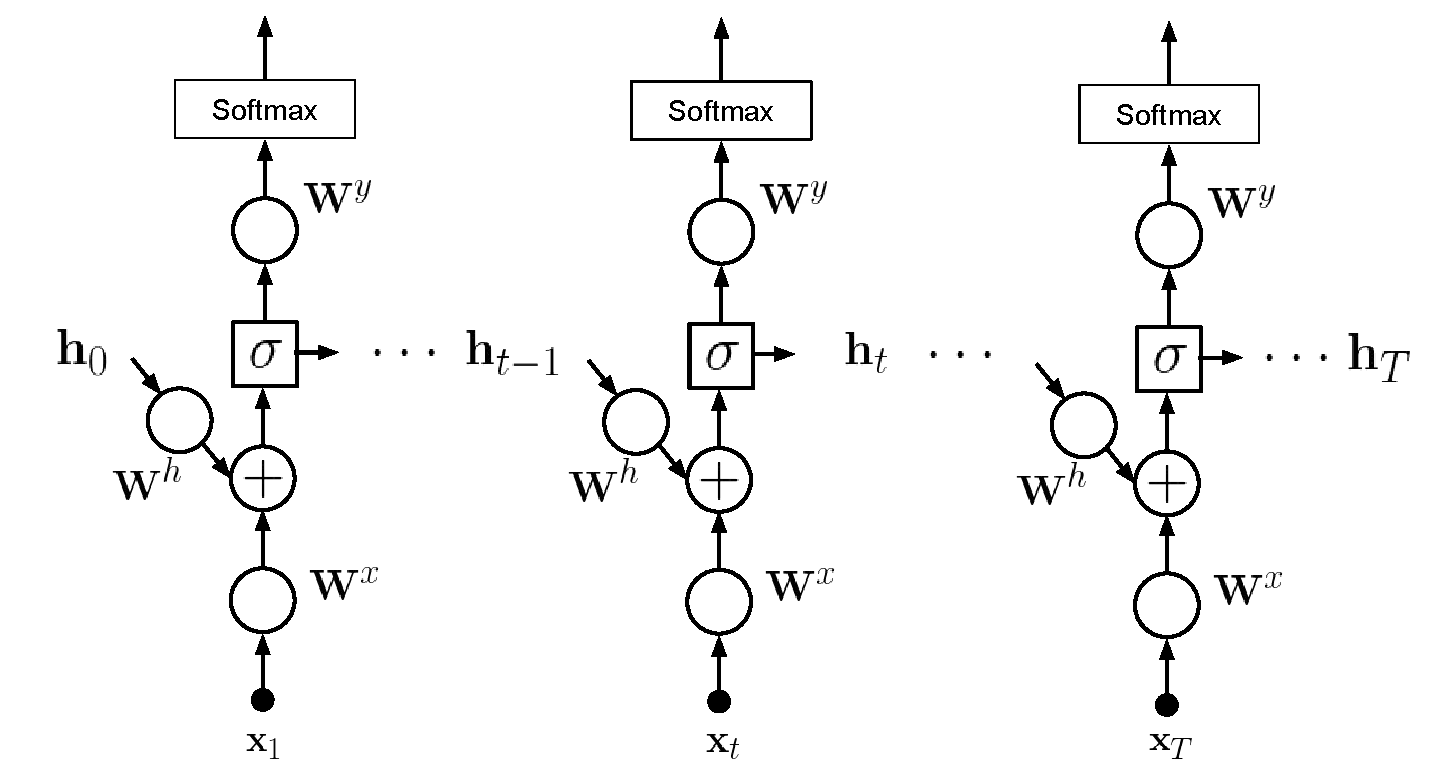
\includegraphics[scale=0.6]{figs/deep_learning/RNN.pdf}
\caption{The simplest RNN can be seen as replicating a single hidden-layer FF
network $T$ times and passing the intermediate hidden variable $\mathbf{h}_t$
across different steps. Note that all nodes operate over vector inputs e.g,.
$\mathbf{x}_t \in \mathbb{R}^I$. Circles indicate matrix multiplications.}
\label{fig:RNN}
\end{figure}

The previous day focused on Feed Forward (FF) networks. These networks are ill
suited to learn variable length patterns since they only accept inputs of a
fixed size. In order to learn sequences using neural networks, we need therefore
to define some architecture that is able to process variable length inputs.
Recurrent Neural Networks (RNNs) solve this problem by unfolding the
computation graph in time. In other words, the network is replicated as many
times as it is necessary to cover the sequence to be modeled. In order
to model the sequence one or more connections across different time instants are
created. This allows the network to have a memory in time and thus capture
complex patterns in sequences. In the simplest model, depicted in
Fig.~\ref{fig:RNN}, and detailed in Algorithm~\ref{algo:rnnforward}, a RNN is
created by replicating a single hidden-layer FF network $T$ times and passing
the intermediate hidden variable across different steps. 

Since RNNs are computation graphs involving the same operations as FF networks,
they can also be trained with backpropagation. However the error is
 propagated over the length of the entire sequence. This often leads to 
numerical problems know as \textit{vanishing} and \textit{exploding} gradients.
A number of solutions are used to mitigate this issue. One simple, yet inelegant,
method is clipping the gradients to a fixed threshold. Another solution is to resort to more complex 
RNN models that are able to better handle long range dependencies and are less
sensitive to this phenomena. It is important to bear in mind, however, that
all RNNs still use backpropagation as seen in the previous day, although it is
often referred as \textit{Backpropagation through time}. 

%What we saw with FF and RNN netwoeksThe only
%difference is that, as the complexity of the computation graph grows, it is
%increasingly difficult to derive individual closed form solutions for each model.
%This is the reason to resort to tools like Theano or TensorFlow, allow us
%to define arbitrary computation graphs and derive the gradients automatically.

\begin{algorithm}[th!]
\label{algo:rnnforward}
   \caption{Forward pass of a Recurrent Neural Network (RNN)}
\begin{algorithmic}[1]

   \STATE {\bfseries input:} Initial parameters for an RNN Input
$\Theta=\{\mathbf{W}^x \in \mathbb{R}^{H \times I}, \mathbf{W}^h \in \mathbb{R}^{H \times H}, \mathbf{W}^y \in \mathbb{R}^{K \times H} \}$ input, recurrent and output transformations respectively.

   \STATE {\bfseries input:} Input data matrix $\mathbf{x} \in \mathbb{R}^{I \times T}$ of size $T$. Initial recurrent variable $\mathbf{h}_0$. 

	\FOR{$t=1$ {\bfseries to} $T-1$}
     \STATE Apply linear transformation combining input and recurrent signals
        $$z_{jt}^h = \sum_{i=1}^{I} W_{ji}^x x_{it} + \sum_{j'=1}^{J} W_{jj'}^h h_{j't-1}$$
     \STATE Apply non-linear transformation e.g. sigmoid (hereby denoted $\sigma()$)
     $$h_{jt} = \sigma(z_{jt}^h)  = \frac{1}{1+\exp(-z_{jt}^h)}$$

	\ENDFOR

\STATE Apply final linear transformation to each of the recurrent variables $\mathbf{h}_1 \cdots \mathbf{h}_T$ 
   $$z_{kt}^y = \sum_{j=1}^{J} W_{kj}^y h_{jt}$$
\STATE Apply final non-linear transformation e.g. softmax 
$$p(y_t=k|\mathbf{x}_{t:}) = \frac{\exp(z_{kt}^y)}{\sum_{k'=1}^{K} \exp(z_{k't}^y)}$$

\end{algorithmic}
\end{algorithm}

\begin{exercise}
\label{exercise:Ex1}
Convince yourself that a RNN is just an FF unfolded in time. Run the NumpyRNN
code. Set break-points and compare with what you learned about backpropagation
in the previous day. 

To work with RNNs we will use the Part-of-speech data-set seen in the sequence
models day.
\begin{python}
# Load Part-of-Speech data 
import lxmls.readers.pos_corpus as pcc
corpus = pcc.PostagCorpus()
train_seq = corpus.read_sequence_list_conll("data/train-02-21.conll", max_sent_len=15, max_nr_sent=1000)
test_seq = corpus.read_sequence_list_conll("data/test-23.conll", max_sent_len=15, max_nr_sent=1000)
dev_seq = corpus.read_sequence_list_conll("data/dev-22.conll", max_sent_len=15, max_nr_sent=1000) 
\end{python}
We will need to redo the indices of
the data so that they are consecutive and cast all data to numpy arrays
of int32 for compatibility with GPUs. This function will also add reverse
indices to recover tag and word from its index word\_dict and tag\_dict  
\begin{python}
# Redo indices 
train_seq, test_seq, dev_seq = pcc.compacify(train_seq, test_seq, dev_seq, theano=True)
# Get number of words and tags in the corpus
nr_words = len(train_seq.x_dict)
nr_tags = len(train_seq.y_dict)
\end{python}

\noindent Load and configure the NumpyRNN. Remember to use reload if you want to modify 
the code inside the rnns module
\begin{python}
import lxmls.deep_learning.rnn as rnns
reload(rnns)
# RNN configuration
SEED = 1234       # Random seed to initialize weigths
emb_size = 50     # Size of word embeddings
hidden_size = 20  # size of hidden layer
# RNN
np_rnn = rnns.NumpyRNN(nr_words, emb_size, hidden_size, nr_tags, seed=SEED)
# Example sentence
x0 = train_seq[0].x
y0 = train_seq[0].y
\end{python}
Compute forward pass and gradients
\begin{python}
# Forward pass
p_y, y_rnn, h, z1, x = np_rnn.forward(x0, all_outputs=True)
# Gradients
numpy_rnn_gradients = np_rnn.grads(x0, y0)
\end{python}

\end{exercise}

\section{The Scan operation in Theano}

Handling variable length computation graphs in an automatic fashion is not simple. 
Theano provides the \textit{scan} function for this purpose. The scan function acts
as a symbolic ``for'' loop. Since, unlike for normal python ``for'' loops, it is not
possible to put a breakpoint in the scan loop, the design of graphs
with scan has to be handled with care. Toolboxes like Keras conveniently abstract
the user from such constructs. However, for complex designs it will be
necessary to be able to use scan or equivalent functions. 

\begin{exercise}
\label{exercise:Ex2}
Understand the basics of scan with these examples. Scan allows you to build
computation graphs with a variable number of nodes. It acts as a python "for"
loop but it is symbolic. The following example should help you understand the
basic scan functionality. It generates a sequence for a given length. Run it
and modify it. Try to arrive at an error and understand what happened.
\begin{python}
import numpy as np
import theano
import theano.tensor as T
theano.config.optimizer='None'

def square(x): 
    return x**2 

# Python
def np_square_n_steps(nr_steps):
    out = []
    for n in np.arange(nr_steps):
        out.append(square(n))
    return np.array(out)


\end{python}
\begin{python}
# Theano
nr_steps = T.lscalar('nr_steps')
h, _ = theano.scan(fn=square, sequences=T.arange(nr_steps))
th_square_n_steps = theano.function([nr_steps], h)

# Compare both
print np_square_n_steps(10)
print th_square_n_steps(10)
\end{python}
The following example should help you understand about matrix multiplications
and passing values from one iteration to the other. At each step, we will
multiply the output of the previous step by a matrix A. We start with an
initial vector s0. The matrix and vector are random but normalized to result on
a Markov chain (this is irrelevant for the use of scan).  
\begin{python}
# Configuration
nr_states = 3
nr_steps = 5

# Transition matrix
A = np.abs(np.random.randn(nr_states, nr_states))
A = A/A.sum(0, keepdims=True)
# Initial state
s0 = np.zeros(nr_states)
s0[0] = 1
\end{python}


\begin{python}
# Numpy version
def np_markov_step(s_tm1): 
    s_t = np.dot(s_tm1, A.T)
    return s_t 

def np_markov_chain(nr_steps, A, s0):
    # Pre-allocate space
    s = np.zeros((nr_steps+1, nr_states))
    s[0, :] = s0
    for t in np.arange(nr_steps):
        s[t+1, :] = np_markov_step(s[t, :])
    return  s   

np_markov_chain(nr_steps, A, s0)
\end{python}

\begin{python}
# Theano version
# Store variables as shared variables
th_A = theano.shared(A, name='A', borrow=True)
th_s0 = theano.shared(s0, name='s0', borrow=True)
# Symbolic variable for the number of steps
th_nr_steps = T.lscalar('nr_steps')

def th_markov_step(s_tm1): 
    s_t = T.dot(s_tm1, th_A.T)
    # Remember to name variables
    s_t.name = 's_t'
    return s_t 

s, _ = theano.scan(th_markov_step, 
                   outputs_info=[dict(initial=th_s0)], 
                   n_steps=th_nr_steps)
th_markov_chain = theano.function([th_nr_steps], T.concatenate((th_s0[None, :], s), 0))

th_markov_chain(nr_steps)
\end{python}
\end{exercise}

\section{A RNN in Theano for Part-of-Speech Tagging}

\begin{exercise}
Complete the theano code for a RNN inside lxmls/deep\_learning/rnn.py. Use
exercise \ref{exercise:Ex1} for a numpy example and \ref{exercise:Ex2} to learn
how to handle scan. Keep in mind that you only need to implement the forward
pass! Theano will handle backpropagation for us. 
\begin{python}
# Instantiate the class
rnn = rnns.RNN(nr_words, emb_size, hidden_size, nr_tags, seed=SEED)
# Compile the forward pass function
x = T.ivector('x')
th_forward = theano.function([x], rnn._forward(x).T)
\end{python}
When working with theano, it is more difficult to localize the source of
errors. It is therefore important to work step by step and test the
code frequently. To debug we suggest to implement and compile the forward pass
first. You can use this code for testing. If it raises no error you are good to
go.
\begin{python}
assert np.allclose(th_forward(x0), np_rnn.forward(x0)), \
    "Numpy and Theano forward pass differ!"
\end{python}
Once you are confident the forward pass is working you can test the gradients
\begin{python}
# Compile function returning the list of gradients
x = T.ivector('x')     # Input words
y = T.ivector('y')     # gold tags 
p_y = rnn._forward(x)
cost = -T.mean(T.log(p_y)[T.arange(y.shape[0]), y])
grads_fun = theano.function([x, y], [T.grad(cost, par) for par in rnn.param])
\end{python}

\begin{python}
# Compare numpy and theano gradients
theano_rnn_gradients = grads_fun(x0, y0)
for n in range(len(theano_rnn_gradients)): 
    assert np.allclose(numpy_rnn_gradients[n], theano_rnn_gradients[n]), \
        "Numpy and Theano gradients differ in step n"
\end{python}

\noindent Finally, it is time to test our network in the task of POS tagging. Lets define
the optimization parameters and compile batch update and prediction
functions

%For this,
%lets first compile a function that does predictions
%\begin{python}
%rnn_prediction = theano.function([x], T.argmax(p_y, 1))
%# Lets test the predictions
%def test_model(sample_seq, rnn_prediction):
%    words = [train_seq.word_dict[wrd] for wrd in sample_seq.x]
%    tags = [train_seq.tag_dict[pred] for pred in rnn_prediction(sample_seq.x)]
%    print ["/".join([word, tag]) for word , tag in zip(words, tags)]
%\end{python}
\begin{python}
# Parameters
lrate = 0.5   # Learning rate
n_iter = 5    # Number of iterations
# Get list of SGD batch update rule for each parameter
updates = [(par, par - lrate*T.grad(cost, par)) for par in rnn.param]
# compile
rnn_prediction = theano.function([x], T.argmax(p_y, 1))
rnn_batch_update = theano.function([x, y], cost, updates=updates)
\end{python}

\clearpage

\noindent To train the newtwork with SGD, you can use the following code for
this purpose
\begin{python}
nr_words = sum([len(seq.x) for seq in train_seq])
for i in range(n_iter):
    # Training
    cost = 0
    errors = 0
    for n, seq in enumerate(train_seq):
        cost += rnn_batch_update(seq.x, seq.y)
        errors += sum(rnn_prediction(seq.x) != seq.y)
    acc_train = 100*(1-errors*1./nr_words) 
    print "Epoch %d: Train cost %2.2f Acc %2.2f %%" % (i+1, cost, acc_train), 
    # Evaluation    
    errors = 0
    for n, seq in enumerate(dev_seq):
        errors += sum(rnn_prediction(seq.x) != seq.y)  
    acc_dev = 100*(1-errors*1./nr_words) 
    print " Devel Acc %2.2f %%" % acc_dev
    sys.stdout.flush()
\end{python}


\end{exercise}


\section{The Importance of Pre-training}

% TODO: Maybe make this about Pre-raining and Dropout?

One of the key insights that has played a role in the rise of deep learning in
NLP tasks is the use of neural word-embeddings. These are just numeric 
representations of words that can be learned from unsupervised data using
simple FF networks such as e.g. skip-grams.

Such representations can be plugged into supervised models such as the RNN that we just
trained to initialize its initial layer. The use of pre-trained embeddings very often leads to
important improvements in performance. 

\begin{exercise}
Test the effect of using pre-trained embeddings. Run the following code to
download the embeddings. Reset the layer parameters and initialize the
embedding layer with the pre-trained embeddings. Then run the training code
from the last exercise.
\begin{python}
# Embeddings Path
import lxmls.deep_learning.embeddings as emb
import os
reload(emb)
if not os.path.isfile("data/senna_50"):
    emb.download_embeddings('senna_50', "data/senna_50")
E = emb.extract_embeddings("data/senna_50", train_seq.x_dict) 
# Reset model to remove the effect of training
rnn = rnns.reset_model(rnn, seed=SEED)
# Set the embedding layer to the pre-trained values
rnn.param[0].set_value(E.astype(theano.config.floatX)) 

# Now re-run SGD training
\end{python}
\end{exercise}

\section{More Complex RNNs: LSTMs}

As previously mentioned, the basic RNN that we saw until now suffers from a
number of drawbacks like exploding or vanishing gradients, and the inability to
model long term dependencies. These deficiencies are solved by more complex
RNNs that include more complex internal logics, and are able to selectively
forget, thus capturing better long term information. The so called Long Short-Term Memory
(LSTM) and Gated Recurrent Unit (GRU) have replaced simple RNNs in most of modern
models. However, they only imply more complex architectures. For an excellent 
visual explanation of the differences between simple RNNs, GRUs and LSTMs please visit 

\begin{verbatim}
http://colah.github.io/posts/2015-08-Understanding-LSTMs/
\end{verbatim}

\begin{figure}[!h]
\centering
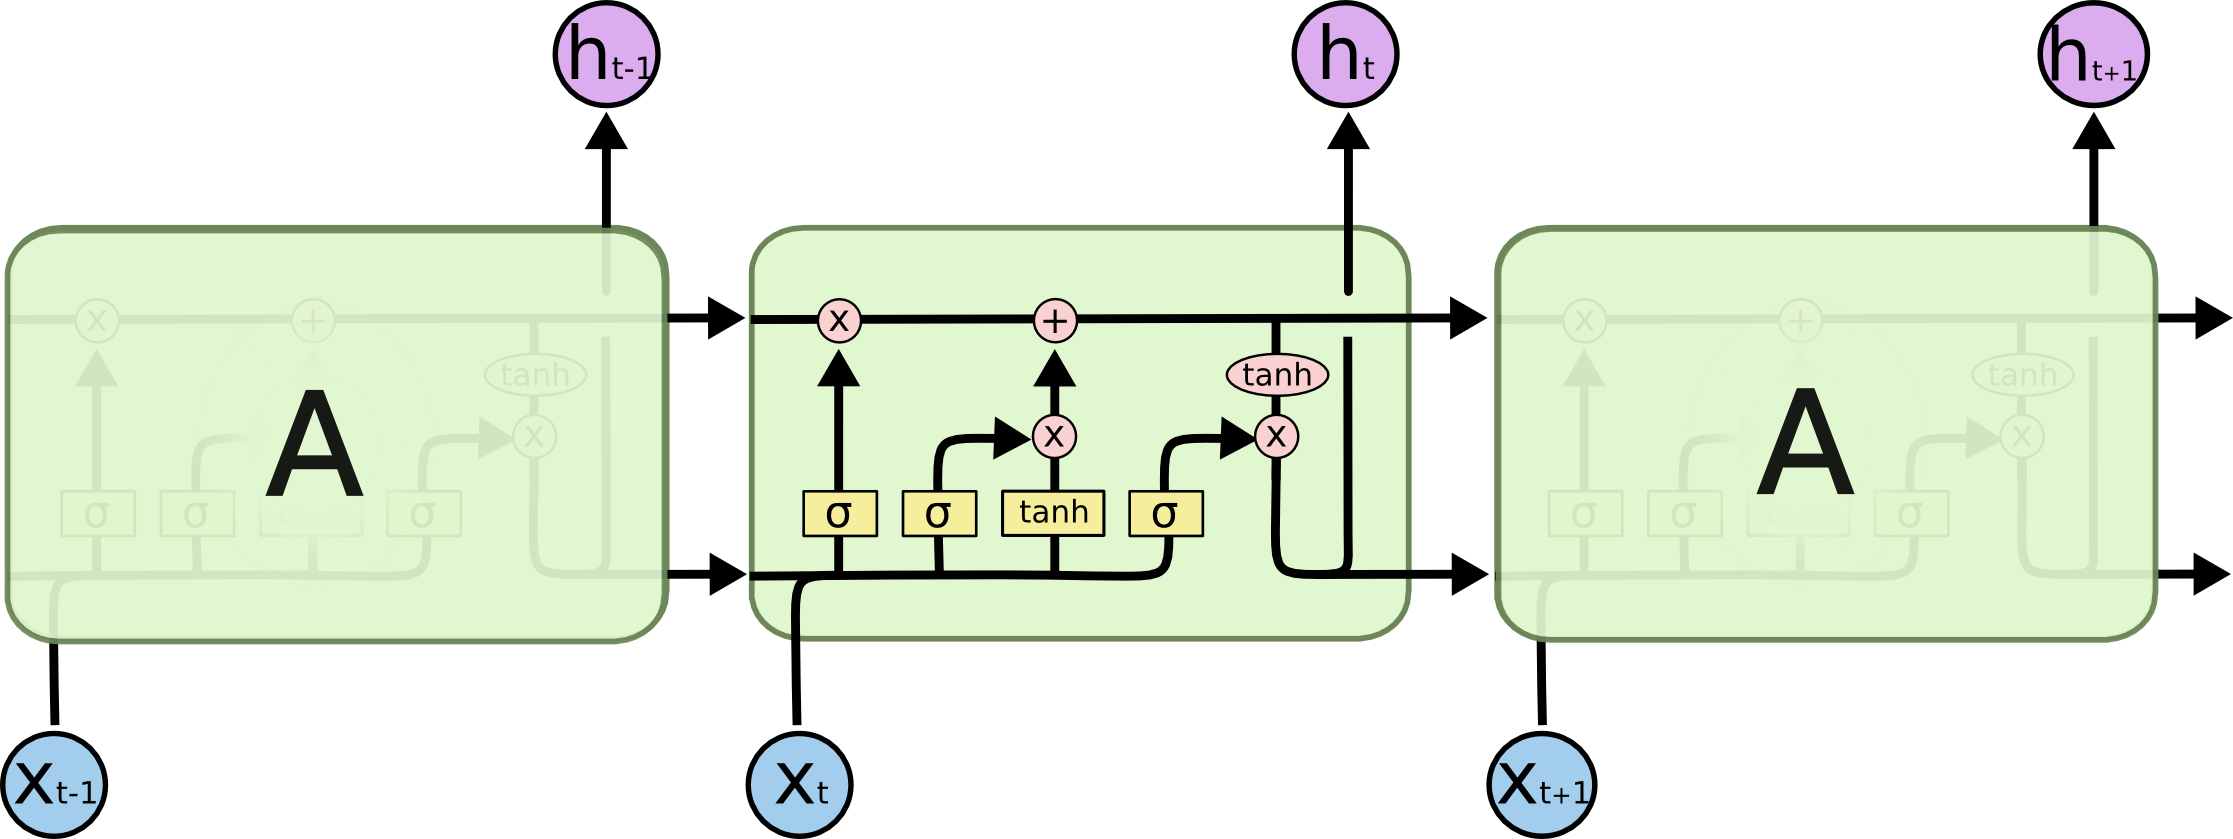
\includegraphics[scale=0.6]{figs/deep_learning/LSTM3-chain.png}
\caption{Detailed explanation of the LSTM internal logic, see source: \url{http://colah.github.io/posts/2015-08-Understanding-LSTMs/}.}
\label{fig:LSTM}
\end{figure}

\begin{exercise}
Convince yourself that LSTMs are just more complex RNNs. Run them, play around
with the hyper parameters and compare the RNN and LSTM classes.
\begin{python}
# Instantiate LSTM
lstm = rnns.LSTM(nr_words, emb_size, hidden_size, nr_tags)
# Compile prediction and bacth update functions
lstm_prediction = theano.function([x], T.argmax(lstm._forward(x), 1))
lstm_cost = -T.mean(T.log(lstm._forward(x))[T.arange(y.shape[0]), y])
# Get list of SGD batch update rule for each parameter
lstm_updates = [(par, par - lrate*T.grad(lstm_cost, par)) for par in lstm.param]
# compile
lstm_batch_update = theano.function([x, y], lstm_cost, updates=lstm_updates)
\end{python}

\begin{python}
nr_words = sum([len(seq.x) for seq in train_seq])
for i in range(n_iter):
    # Training
    cost = 0
    errors = 0
    for n, seq in enumerate(train_seq):
        cost += lstm_batch_update(seq.x, seq.y)
        errors += sum(lstm_prediction(seq.x) != seq.y)
    acc_train = 100*(1-errors*1./nr_words) 
    print "Epoch %d: Train cost %2.2f Acc %2.2f %%" % (i+1, cost, acc_train), 
    # Evaluation:
    errors = 0
    for n, seq in enumerate(dev_seq):
        errors += sum(lstm_prediction(seq.x) != seq.y)  
    acc_dev = 100*(1-errors*1./nr_words) 
    print " Devel Acc %2.2f %%" % acc_dev
    sys.stdout.flush()
\end{python}
\end{exercise}
